\documentclass[man]{apa2}
\usepackage{pslatex}
\usepackage{amssymb}
\usepackage{graphicx}
\usepackage{color}
\usepackage{covington}
\usepackage[usenames,dvipsnames]{xcolor}

\title{Pragmatic contrast helps preschoolers learn category structure}

\twoauthors{Alexandra C. Horowitz}{Michael C. Frank}
\twoaffiliations{Department of Psychology, Stanford University}{Department of Psychology, Stanford University}


\abstract{Children learn some cultural information through explicit instruction (e.g., ``put the fork on the left of the plate'') and generic statements (``forks go on the left''), but not all norms are stated directly. We investigate the idea that adults and children may learn generalizable knowledge via Gricean pragmatic inferences about why speakers choose a particular way to convey a message. We focus on the case of learning relevant dimensions of category variability based on the descriptions speakers choose. For example, if a parent says, ``that�s a salad fork,'' he is implicitly revealing that forks vary in the foods they are intended for (and that most other forks are likely used for non-salad items). 

Contrastive word choices�particularly (but not limited to) adjectives�can help identify the speaker�s intended referent in the current context (selecting the desired fork) and can jointly signal generalizable knowledge (forks are associated with meal courses). In our work, we examine whether children are sensitive to adjective modifiers as markers of important dimensions of contrast for unfamiliar categories.  

In our experiments, we introduced children to ambiguous novel objects that could be generalized along several different dimensions of variation and asked whether the pragmatics of adjective use allowed the children to choose which dimension was relevant for generalization. On each trial, we presented and contrastively named a single object (e.g., �a tall glorp�) and then showed children two similar objects that each differed by a single property (e.g., same size but different color, or same color but different size).  We then asked children what they thought most members of the category looked like.  By age 3.5, preschoolers were more likely to select the property contrast (e.g., the short shape) for familiar scalar opposites (size and state features).  By age 4.5, children also made contrast judgments for non-scalar properties (color). 

Our findings suggest that in their preschool years, children are gaining the ability to learn from speakers� word choices.  Rather than matching the named description they heard in our task (e.g. hearing �tall� and selecting another tall shape), children were able to select the object that contrasted with the named property (the short shape). Sensitivity to implied contrasts of the sort we study here can help children access opportunities for learning about the world, allowing them to acquire knowledge implicitly from adults� descriptions as well as through explicit teaching.

~\\

Keywords: pragmatics; generics; language development; adjectives; contrast}

\shorttitle{Discourse as a Cue for Inferring Reference}
\rightheader{Discourse as a Cue for Inferring Reference}

\acknowledgements{Special thanks to the staff and families at the Bing Nursery School and the Children's Discovery Museum of San Jose. This work supported by a John Merck Scholars Fellowship to MCF. Earlier versions of this work were presented to the Cognitive Science Society in \citeA{horowitz2012} and \citeA{horowitz2014}.

~\\

\noindent Address all correspondence to Alexandra C. Horowitz, Stanford University, Department of Psychology, Jordan Hall, 450 Serra Mall (Bldg. 420), Stanford, CA, 94305. Phone: 650-721-9270. E-mail: \texttt{ahorowit@stanford.edu}}

\begin{document}

\maketitle                            


\section{Introduction}

A large body of cultural knowledge is never taught�or even described�it is simply presupposed by the way adults talk and act. How do children acquire such knowledge? Our work investigates one possible hypothesis: Children make inferences about adults� actions (linguistic and non-linguistic) and work backwards to infer the perceived norm or state of the world that motivates these actions \cite{shafto2012}. We test this hypothesis using a simple case study: learning to generalize novel words via the contrastive descriptions that speakers use. 

%Our work connects mechanisms of pragmatic inference, which have been well-studied in language development, with processes of cultural learning and generalization. We show that children can figure out that naming a �tall glorp� implies that most glorps are shorter. The same mechanism might also allow them to infer (usefully) that the term �cognitive scientist� implies the existence of other types of scientists, or to infer (negatively) that �female scientist� implies that most scientists�at least in the mind of the speaker�are not female. Thus, pragmatic inferences of the type we study here may constitute an important mechanism of transmission for cultural knowledge. 

From early word learning, children may use the principle of contrast -- that a contract in form conveys a contrast in meaning \cite{clark1987} -- to infer that modified nouns phrases convey different information than that of bare nouns.  


\section{Experiment 1a: scalar properties (opposites)}

We first investigated preschoolers' sensitivity to implied contrasts using familiar scalar properties.  We reasoned that children may be more likely to infer contrast information when they are able to recognize that the adjective used is a member of an opposite pair (e.g. tall--short). We designed a task in which the choice of adjective was the only informative cue to implicit referential contrast.  If children use adjective information to generalize, they should identify other category members by matching this property.  If they use adjective information to make inferences about implied contrasts, they should identify other category members by whether they contrast along the stated dimension.  We found that young 3--year--olds were unable to systematically recognize category membership through speakers' adjective choices, but age 3.5, children showed sensitivity to implicit dimensions of contrast contained in word choice.  



\section{Methods}


\subsection{Participants}
We recruited a planned sample of 96 children into four age groups: 3.0--3.5 years (n=24, NUMBER girls, mean age 3 years 3 months), 3.5--4.0 years (n=24, NUMBER girls, mean age 3 years 9 months), 4.0--4.5 years (n=24, NUMBER girls, mean age 4 years 3 months), and 4.5--5.0 years (n=24, NUMBER girls, mean age 4 years 8 months).  About half of the sample was recruited from the Bing Nursery School at Stanford University (n=52) and half was recruited from the San Jose Children's Discovery Museum (n=44), divided approximately evenly across age groups.\footnote{Some variability in age and gender counts across locations arises from our commitment to recruit inclusively at the Children�s Discovery Museum.  In our partnership, we invite any interested visitors to participate in our studies rather than prescreening children to meet our language requirements or counterbalance all demographic factors \cite{callanan2012}.}


%\foonote{Some variability in age and gender counts across locations arises from our commitment to recruit inclusively at the Children�s Discovery Museum.  In our partnership,  we invite any interested visitors to participate in our studies rather than prescreening children to meet our language requirements }


At the Children's Discovery Museum, parents were asked to fill out a short demographic form about their children's language background.  Only children who were reported to hear English at least 75\% of the time were included in the final sample.  [FILL IN NUMBER] were excluded from analysis based on this criterion\footnote{Bing Nursery School is an English language preschool, and children included in the sample were fluent speakers of English. Children from Bing Nursery School and the Children's Discovery Museum are roughly equated demographically in terms of language exposure, ethnic backgrounds, and parental education, as reported by parents from each location.  Both locations were mainly composed of educated middle class families.  We tested for effect of location, and found no differences across children tested at either location.}.  Children recruited from the museum received a sticker and a certificate for their participation.  An additional [FILL IN NUMBER] were excluded for not completing all four experimental trials, and [FILL IN NUMBER] were dropped from analysis due to interference from parents or siblings interrupting the study procedure. 

[ADD IN GENDER INFO] [ADD IN OTHER MUSEUM DEMOGRAPHIC INFO?]

\subsection{Stimuli}

Children were read a storybook with colorful clipart images.  Each child participated in two training trials and four test trials.  Training trials featured three pictures of familiar items, only two of which shared a contrast property (e.g. chocolate milk, plain milk, and orange juice).  For the test trials, children were shown sets of three similar images: a novel exemplar shape followed by one picture that differed from the exemplar only by size, and one picture that differed from the exemplar only by a feature contrast (e.g. broken versus unbroken) (See Figure \ref{fig:inanimate_demo}). The named size contrasts were \emph{small} (vs. big), \emph{long} (vs. short), \emph{tall} (vs. short), and \emph{short} (vs. long).  The named feature contrasts were \emph{broken} (vs. unbroken), \emph{pointy} (vs. smooth), \emph{dirty} (vs. clean), and \emph{wet} (vs. dry).  To ensure that children were familiar with the contrasts used, a posttest of pictures exemplifying each of these properties was included in a posttest.  Children were able to recognize the contrasts used in our task, with average accuracy of 90\% for 3--3.5 year--olds, 95\% for 3.5--4.0 year--olds, 96\% for 4.0--4.5 year--olds, and 98\% for 4.5--5.0 year--olds.  

\begin{figure} 
  \begin{center} 
    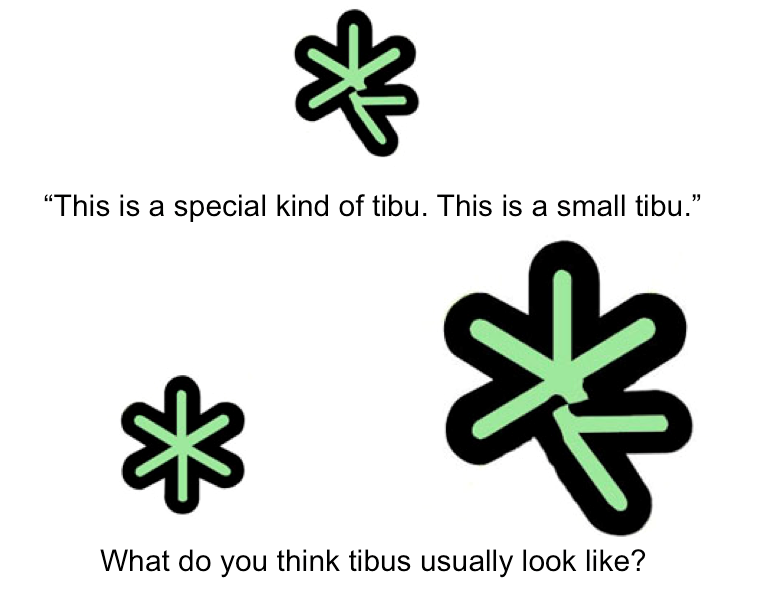
\includegraphics[width=4in]{figures/inanimate_demo.png} 
    \caption{\label{fig:inanimate_demo} Example of a test trial for Experiment 1a.  Children were introduced to an exemplar shaped described with either a size or feature adjective.  They were then shown two images, one that differed from the exemplar by size an done that differed from the exemplar by a feature and were asked to point to which picture they thought was also a member of the same category. } 
  \end{center} 
\end{figure}	



\subsection{Procedures}

The experimenter read the storybook with children individually in a quiet room at either Bing Nursery School of the San Jose Children's Discovery Museum.  At the museum, parents accompanied children and sat either next to or behind the child.  Siblings were sometimes also present, and were offered quiet activities such as coloring or reading. 

To begin the book, children were introduced to a character named Allen the Alien who was visiting planet Earth.  Children then participated in two training trials containing familiar items to teach Allen about some things on Earth and get children used to the study design.  Training trials featured adjectives other than those used in critical trials, and training pictures displayed only one relevant contrast choice.  For example, children were shown a picture of chocolate milk followed by two pictures, one of plain milk and one of orange juice.  Children were told, ``This is a special kind of milk.  This is \emph{chocolate} milk.  What does milk usually look like?  What does most milk look like?" and prompted to point to the picture.  On the rare occasion that children answered incorrectly, the experimenter repeated the statements and encouraged children to point to the correct picture until they answered correctly.  

After the training trials, children participated in four test trials.  For each test trial, children were shown a picture of a single exemplar (e.g. a small broken tibu, see Figure \ref{fig:inanimate_demo}) and told something about it, e.g. ``This is a special kind of tibu.  This is a small tibu."  They were then shown two similar pictures, one that differed from the exemplar only by size (i.e. a big broken tibu) and one that differed from the exemplar only by a feature (i.e. a small fixed tibu), and were asked ``What do you think tibus usually look like?  What do you think most tibus look like?".  They were prompted to select one of non-exemplar images.  Two of the four trials used size adjectives (e.g. ``This is a small tibus") and two of the trials used feature adjectives (e.g. ``This is a broken tibu"). The order of trial items varied across two lists, each of which was counterbalanced for adjective type and picture order.  Adjectives were focused using contrastive stress.  The experimenter averted her gaze while children pointed to their responses.  Responses were coded online and double-coded offline using a video recording of the testing session.  The task took about ten minutes to complete. 

\subsection{Results}

We categorized a response as a correct contrast inference if children selected the item that differed from the exemplar along the referenced dimension (i.e. they chose the short item if the exemplar was referred to as ``tall", but the clean item if it was referenced as ``dirty").  We found that preschoolers' sensitivity to contrast information implicit to adjective choice increased from ages 3--6 years of age.  The youngest children in our sample did not demonstrate systematic inferences to adjective information; 3--3.5 year--olds selected the adjective match and the adjective contrast at chance levels when selecting another example of a category member with the referent.  However, by age 3.5, children predictively selected the contrasting property to the adjective named.  Within the early preschool years, children appear to gain sensitivity in assessing speakers' word choice information and the implicit contrast information it may contain. 

Overall, we see that, although even the youngest children in our sample were familiar with the adjectives and their contrast alternatives used in our task, children younger than age 3--and--a--half were unable to reliably use adjective information to infer implicit contrast information.  However, children ages 3.5--4.0 were reliably above chance in selecting the contrast property when size terms were used, and marginally above chance when feature contrasts were used.  Children ages 4.0--4.5 and 4.5--5.0 were reliably above chance in selecting the property contrast across both feature and size terms.  

We analyzed our results using a logistic mixed model, predicting correct responses as an interaction between age and contrast type with random effects of participant and shape.  Children increasingly made more correct contrast judgments with age ($\beta = 1.51$, $p < .0001$).
% There was a significant effect of age, such that children increasingly made more correct contrast judgments with age ($\beta = 1.51$, $p < .0001$).   
  There was no significant effect of contrast type (feature vs. size adjectives), and there was no interaction between age and contrast type, suggesting that participants across ages did not differ in their responses to different property types.  Overall, these analyses show that children demonstrate an increasing sensitivity to implicit contrast information from adjectives.  


Our results indicate that preschoolers are gaining sensitivity to the implications of word choice from ages 3--5 years; by age 4, children were reliably able to use adjective information to infer implied contrasts informing category membership.  We next wanted to determine whether children recognize the informativeness of adjective use across additional, non--scalar properties.  By extending our design to other adjective types, we could examine whether children's early success is due to familiarity with the scalar contrasts used, or whether children assume contrast information from adjective use more generally.  In Experiment 1, we wanted to make the cues to contrast as salient as possible by using familiar opposite pairs (e.g. small--big, wet--dry), but it is unclear whether children's success was due to recognition of clear alternatives with these scalar properties, or whether children exhibit sensitivity across other categories without definite alternatives.  In order to investigate children's sensitivity to adjective choice more generally, we next turned to extending our design to familiar non-scalar property contrasts.  We examined children's contrast inferences about color and pattern terms, both of which are familiar to children and may convey property contrast information, yet use of a color or pattern term does not indicate contrast with a particular opposite term (e.g. ``red" may indicate that an item can vary by color, but it does not imply what an alternative color should be).  If children are sensitive to implicit contrast information across property types, they should again select the item varying along the named property even when non-scalar items are used in our task. 


\begin{figure}[t] 
  \begin{center} 
    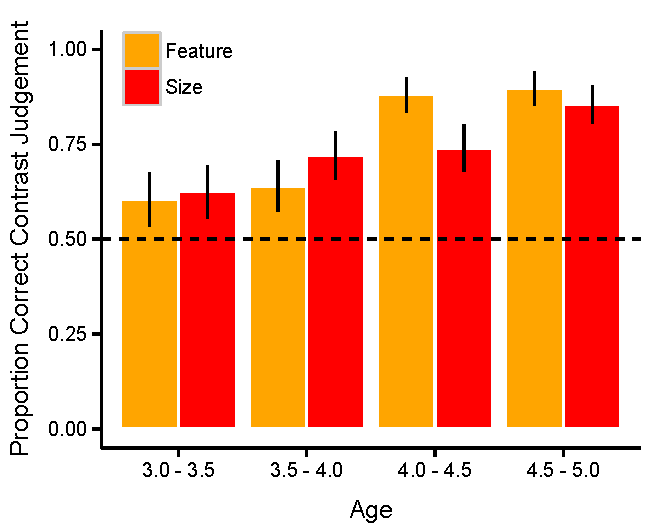
\includegraphics[width=3.5in]{figures/inanimate.pdf} 
    \caption{\label{fig:inanimate} Preschoolers' mean proportion correct performance in Experiment 1b. Yellow bars depict feature adjective trials and red bars depict size trials. The dashed line represents chance (0.5). Error bars represent standard error.}
    %95\% confidence intervals.} 
  \end{center} 
  % \vspace{-2.0ex} 
\end{figure}	



\section{Experiment 1b: non-scalar properties (colors)}
In Experiment 1a, we found that preschoolers rapidly gained sensitivity to implied contrast information from speakers� use of scalar adjectives.  These findings suggest that young chidden are learning to pick up on marked information conveyed by word choices.  They were able to process the property information not simply as a descriptive statement, but as an informative cue to underlying property information about other category members.  In other words, by age 4, they recognized that a size term conveys that size is a variable dimension of interest, while a feature term conveys that the feature dimension is a variable dimension of interest.  In our first experiment, we begin with familiar opposites to help make contrast inferences most accessible to children. In Experiment 1b, we extended our design to include familiar non-scalar properties: color terms.  We contrasted size and color descriptions to examine whether children still make contrast inferences for modifiers that do not have specifically implied opposites. 

\subsection{Participants}
A new planned sample of 48 four-year-old children from the Bing Nursery School at Stanford University. Twenty-four were age 4.0 -- 4.5 (mean age 4 years 2 months) and 24 were age 4.5 -- 5.0 (mean age 4 years 10 months). 

\subsubsection{Stimuli}
A similar triad task was used as in Experiment 1a, but triads were modified to contrast by color and size.  We used alien creatures instead of inanimate shapes in order to make the color category membership more salient to children.  A sample triad is shown in Figure \ref{fig:alien_color_demo}.  Children participated in four unique test trials and two additional unique unmodified baseline trials.  These baseline trials were identical to the experimental trials except that no adjective was included in the speakers� descriptions.  Instead, children were told that, e.g. ``This is a special kind of glorp. This is a glorp.�� and asked to make a selection between the picture that varied by color or by size. 

\begin{figure} 
  \begin{center} 
    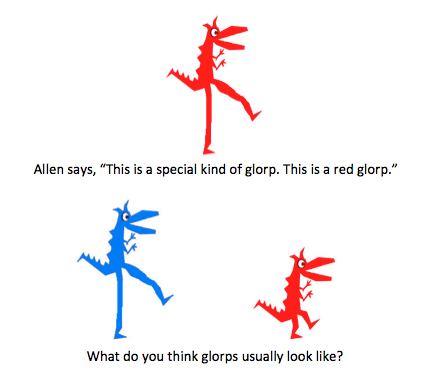
\includegraphics[width=4in]{figures/alien_color_demo.png} 
    \caption{\label{fig:alien_color_demo} Example of a test trial for Experiment 1b.  Children were introduced to an exemplar shaped described with either a size or color adjective.  They were then shown two images, one that differed from the exemplar by size an done that differed from the exemplar by a color and were asked to point to which picture they thought was also a member of the same category. } 
  \end{center} 
\end{figure}	

\subsection{Procedures}
Procedure was identical to Experiment 1a, with the addition of two unmodified baseline trials.  We included these two no-adjective trials in order to determine whether there was a tendency for children to prefer to select pictures that match or varied by one property over the over (e.g. color versus size).  Were were unable to measure a property preference in Experiment 1a because the feature contrasts all varied.  In Experiment 1b, we had the opportunity to measure consistencies between overall color and size selections. 

\subsection{Results and Discussion}
Preschool-aged children did show sensitivity to the implications of adjective use.  Overall, preschoolers could pick out adjective information as marking an implied contrast dimension. Nevertheless, we saw an interesting developmental trend in the data (Figure \ref{fig:res5}).

We analyzed our results using a logit mixed model, predicting correct responses as an interaction between age (older vs. younger) and contrast type with random effects of participant and alien type. There was a significant effect of age, such that older children performed better than younger children ($\beta = -2.06$, $p < .001$).  There was also a significant interaction between age and contrast (color or size) such that older children performed above chance for both color and size trials, and younger children responded above chance for size trials but were only at chance for color trials ($\beta = -3.25$, $p < .01$). Overall, this analysis suggested weak responding by the younger 4s with successes by the older 4s. 

To ensure that performance differences were not due to unfamiliarity with the color and size terms, we ran a posttest with a subset of children for each age group (n=13 younger, n=12 older). Younger children produced the correct size term over 80\% and color terms 95\% of the time.  Older children's production was 94\% for size and 99\% for color. These data suggest that younger children's lower performance on color trials was not a result of not knowing their color words.

Baseline responses also indicated a significant developmental change. While younger 4s chose color-matching targets 71\% of the time on the baseline trials, older 4s chose color-matching targets 38\% of the time. To examine this effect, we replotted our data by proportion of trials on which the color-matching target was chosen (Figure \ref{fig:baserate}). A correct pattern of responding for a color trial would be choosing the size match (hence success on a color trial would be below 50\% in Figure \ref{fig:baserate}), while a correct response on a size trial would be choosing the color match (above 50\%). Replotted in this manner, we can see that younger 4s are modifying their responses only slightly for color trials and not at all for size trials, while older 4s modify their responding slightly for color trials and considerably for size trials. 

We captured this pattern with a second logit mixed model, this time predicting choice of color-matching target as a function of trial type (including baseline), age group, and their interaction. In this analysis, we saw that younger children had a significant bias for color ($\beta = 1.32$, $p = .004$), and a trend towards differential responding in color trials ($\beta = -.83$, $p = .09$). There was a significant coefficient on older children's bias, indicating more size responding ($\beta = -2.02$, $p = .002$), as well as a significant interaction for size trials, indicating success in overcoming this baseline effect ($\beta = 1.76$, $p = .04$), but only for size trials. Thus, both groups showed some bias in their responding, but older 4s were better able to overcome that bias---at least for size---and make inferences about why a particular adjective was produced. 

To summarize: Even within the narrow age range of our sample, there was a developmental difference between performance on color and size adjective trials.  Although children at both ages were sometimes able to make contrast inferences, the ability to make these inferences clearly depended on the category of the adjective being used. 

\begin{figure}[t] 
  \begin{center} 
    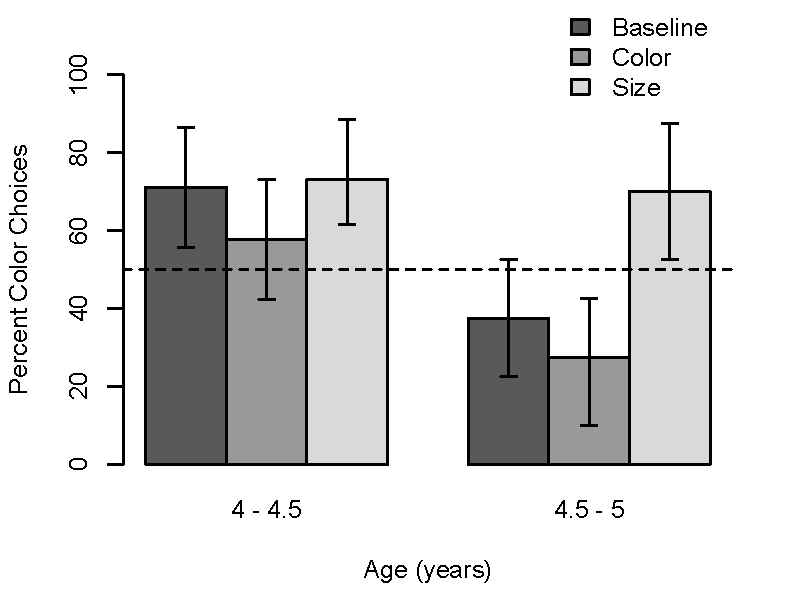
\includegraphics[width=3.7in]{figures/baselineplot.pdf} 
    \caption{\label{fig:baserate} Mean percent color choices for all trials in the three trial types by the children in Experiment 4. Error bars show 95\% confidence intervals.} 
  \end{center} 
  % \vspace{-2.0ex} 
\end{figure}

\section{Experiment 1c: adults performance}
We found developmental differences in 4-year-olds� inferences about speakers� use of scalar versus non-scalar properties.  Color terms are produced more often than other types of adjectives, and it is possible that color terms do not convey the same contrastive information as other modifiers.  We wondered whether adults would show the same pattern of performance and make fewer contrast inferences for color terms than scalar opposites.  Unlike children, adults robustly selected the property contrast for both scalar and non-scalar properties, suggesting that by adulthood, language users infer implied contrast information for both types of modifies, but recognizing opportunities across all modifiers may come with experience. 

\subsubsection{Participants}

A planned sample of 128 (FIX THIS FOR COMBINING EXPERIMENTS) adult participants was recruited from Amazon's Mechanical Turk online crowd-sourcing service.  Three subjects were excluded for failing to complete the task. All participants reported that they were native speakers of English and were informed that the task was designed for children.  

\subsubsection{Stimuli}

Adults participated in a single trial featuring one of the same triads as used with children (e.g. Figure \ref{fig:inanimate_demo}). 

\subsubsection{Procedures}

Participants read a story online in which a cartoon character, Allen the Alien, introduced them to a novel shape from outer space and said something about it, e.g. ``This is a special kind of tibu.  This is a [broken] tibu.'' Half of participants were presented with a feature adjective (e.g. ``broken'') and half were presented with a size adjective (e.g. ``small'').  They were then shown the two test shapes and asked, ``What do you think [tibus] usually look like?'', and prompted to select one of the two images.  We measured the proportion of participants who selected the picture that contrasted with the named property. 


\subsection{Results and Discussion}

Responses were coded as correct if participants selected the shape that differed along the referenced dimension.  In other words, we considered a response to be a correct contrast judgement if the participant selected the shape that differed by feature in feature adjective trials (e.g. heard ``broken'' and selected the shape that was unbroken), and differed by size in size adjective trials (e.g. heard ``small'' and selected the shape that was big).  

ADD IN COLOR DATA!!! 

Participants selected the contrasting dimension more often than chance and at nearly identical rates for both adjective types ($p < .001$ in exact binomial tests for feature and size terms; see Figure \ref{fig:adults_plot}).  Our results indicate that participants used the adjective referenced to make inferences about properties of novel category members, suggesting that adjectives are informative indicators of relevant property information to adults.  They were able to consider the labeled property in order to infer that other novel category members are likely to differ along the referenced dimension. 

Adults had no difficulty making contrast inferences for either the scalar or non-scalar terms.  It appears that children�s difficulty inferring implied contrasts from color terms may arise from a lack of experience considering how and why color terms are used. 



\section{Experiment 2a}
In our first set of experiments, we found that adults consistently made contrast inferences from adjective use, while preschoolers were more likely to recognize contrast for terms with familiar opposites than non-scalar color terms.  These results suggest that children are gaining sensitivity to how speakers mark relevant property information.  They may begin by appreciating that scalar opposites are paired, and that use of one term (e.g. \emph{wet}) implies contrast with its opposite (i.e. \emph{dry}). It may take greater experience with other types of descriptions to recognize implied contrast information for non-scalar properties such as color.  We next wanted to investigate the robustness of children�s contrast inferences for opposite terms.  In our first experiments, we tried to make the cues to contrast as strong as possible by conveying contrastive language in our carrier phrase.  In Experiment 2, we eliminated all cues to contrast except for the adjective used: instead of hearing ``This is a special kind of tibu. This is a [small] tibu,'' children instead heard the stripped down expression ``This is a tibu. This is a small tibu.'' This change allowed us to examine children�s sensitivity implied contrast from scalar terms without the the support of other pragmatic cues. 

\subsection{Participants}
A new sample of 48 children was recruited from Bing Nursery School.  Because of the presumed increased difficulty of this task, we recruited children from the old age groups: 4.0- to 4.5-year-olds (M = 4;3) and 4.5- to 5.0-year-olds (M = 4;8).  ADD REST OF INFO HERE

\subsection{Stimuli}
Stimuli were identical to Experiment 1a.  

\subsection{Procedures}
Procedures were identical to Experiment 1a with the exception that the referential phrase was minimized by removing the phrase ``special kind of'' to reduce contrast cues other than the adjective.  Instead, they heard only ``This is a [tibu]. This is a [broken tibu],'' isolating the adjective as the only available indicator of category membership.

\subsection{Results and Discussion}

Although preschoolers showed increasing contrast selections from adjective use with age in Experiment 1b, they were essentially at chance when the contrastive language framing was removed.  We analyzed our results using a logistic mixed model, predicting correct responses as an interaction between age and contrast type with random effects of participant and shape, and we found no significant effects and no significant interaction. In post-hoc followup tests, older 4s showed a significant feature contrast bias ($p  = .001$, exact binomial test), but this contrast was not reliable in the full model when controlling for participant and item effects, and may have been driven primarily by the ``broken'' and ``clean'' items. Although adults remained attentive to implicit contrast information in both the contrastive language and adjective only framings, children performed substantially worse without the additional linguistic cues to guide their contrast judgements.  

UPDATE THIS INFO WITH LAST FEW KIDS


\begin{figure}[t] 
  \begin{center} 
    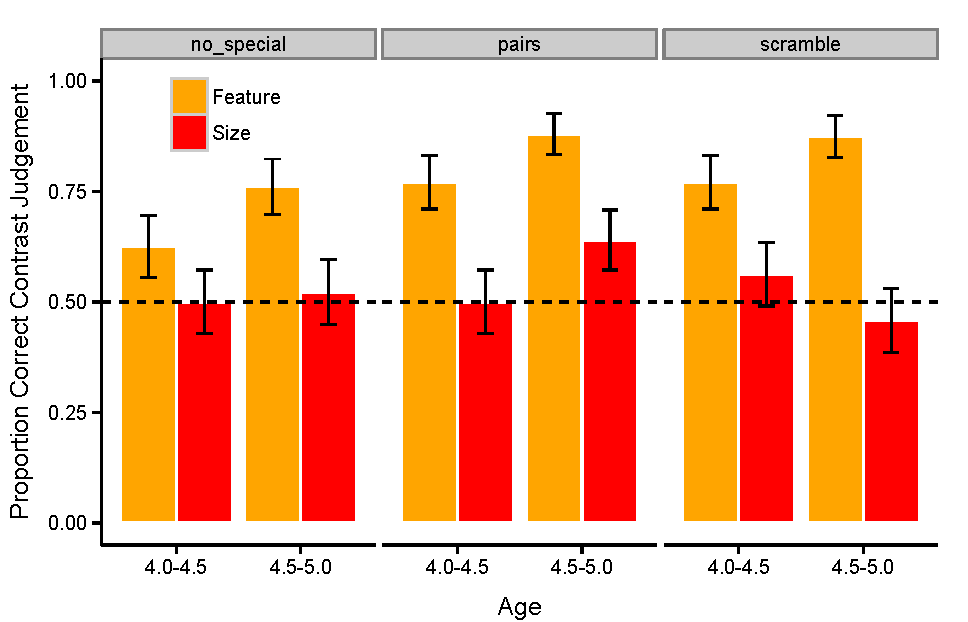
\includegraphics[width=6in]{figures/training_results.pdf} 
    \caption{\label{fig:training_results} Preschoolers' mean proportion correct performance in Experiments 2b and 3.  Feature adjective trials are plotted in yellow and size trials in red. The dashed line represents chance (0.5). Error bars show standard error.}
  \end{center} 
  % \vspace{-2.0ex} 
\end{figure}


\section{Experiment 2b}

We found that children�s contrast selections were dramatically reduced when the contrasting framing cues were removed.  These results suggest that children may rely on additional cues to support contrastive interpretations early on before spontaneously making inferences from adjectives alone.  We next turned to see whether children�s performance matches those of adults. 

\subsection{Participants}
A new planned sample of 128 adult participants were recruited from Amazon's Mechanical Turk online crowd-sourcing service.  Two subjects were excluded for failing to complete the task. All participants reported that they were native speakers of English and were informed that the task was designed for children.  

\subsubsection{Stimuli}
Stimuli were identical to Experiment 1c. 

\subsubsection{Procedures}
Procedures were identical to 1c except that only the feature/size trials were included, and the referential statement was reduced by removing the phrase ``special kind of'' so that listeners heard only ``This is a [tibu]. This is a [broken tibu].''  


\subsection{Results and Discussion}
As above, we measured the proportion of correct contrast judgments for which participants selected the test picture that differed along the referenced property dimension.  Adults performance was significantly about chance ($p < .001$ in exact binomial tests for feature and size terms) and did not differ by adjective type.  They showed only a slight decrease in performance in this adjective only framing from the contrastive language framing in Experiment 1c (see Figure \ref{fig:adults_plot}).  These results indicate that adjective use in our task is a strong indicator of relevant property information of novel category members for adults.  Their nearly equal performance across Experiment 1a and 2a suggests that adjectives provided salient cues to implicit contrast dimensions on their own without the necessity of additional semantic support. 


	
\begin{figure}[t] 
  \begin{center} 
    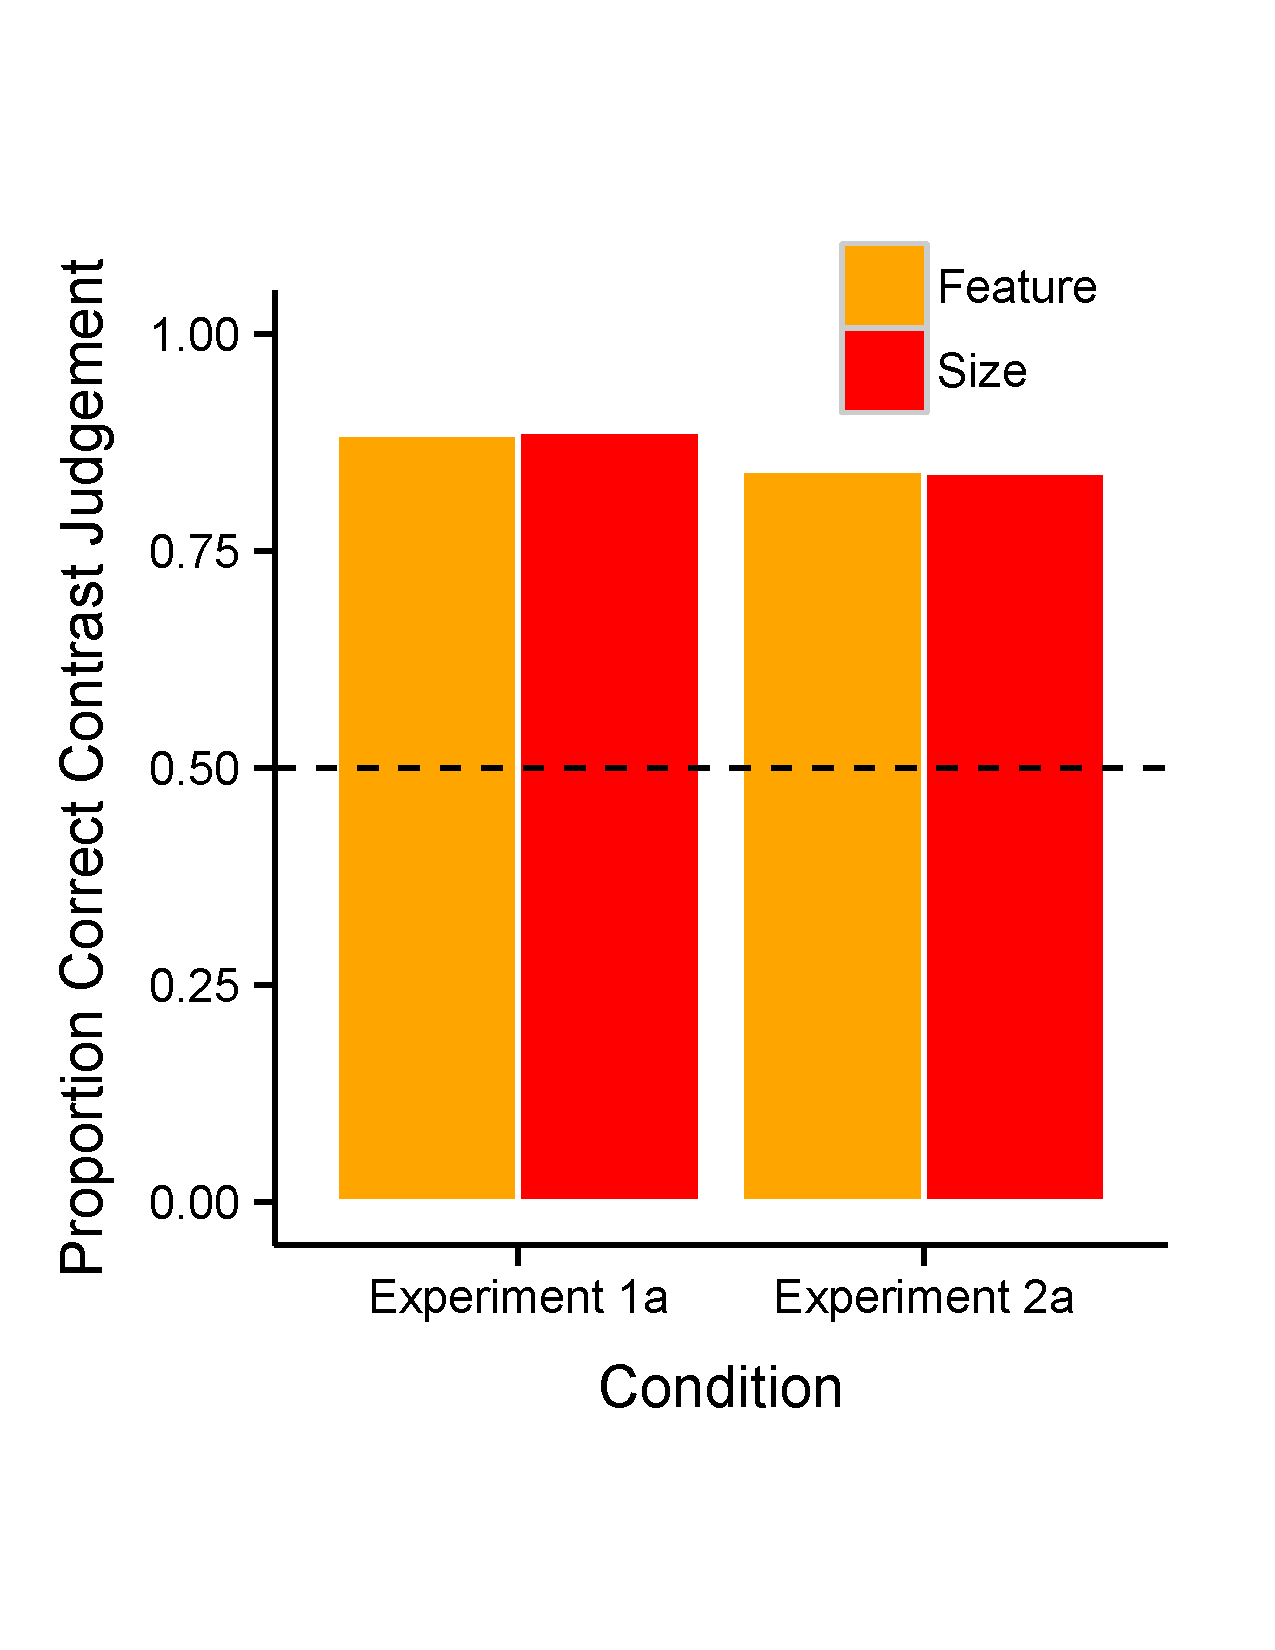
\includegraphics[width=3in]{figures/adults2.pdf} 
    \caption{\label{fig:adults_plot} Adults' mean proportion correct performance in Experiments 1a and 2a. Feature trials are plotted in yellow and size trials in red. The dashed line represents chance (0.5). }
    %Error bars represent 95\% confidence intervals.} 
  \end{center} 
  % \vspace{-2.0ex} 
\end{figure}	



\section{Experiment 3} 



%Although children succeeded in forming contrast inferences from adjective with in the contrastive language framing (Experiment 1b), they had difficulty when the adjective was provided on its own without other cues to contrast (Experiment 2b). 

In Experiment 3, we provide a test of the linguistic alternatives hypothesis by increasing preschoolers' access to the relevant lexical alternatives.  Before the experimental procedure, the experimenter read a seemingly unrelated book featuring the opposites referenced in the test trials (see Figure \ref{fig:training_demo}).  This exposure to linguistic alternatives boosted older 4-year-olds' contrast selections. 

\subsection{Methods}

\subsubsection{Participants}

A new sample of 38 children from Bing Nursery School. Participants were grouped into two age groups: 4.0- to 4.5-year-olds (M = 4;3) and 4.5- to 5.0-year-olds (M = 4;8).

\subsubsection{Stimuli}

Stimuli were identical to Experiment 1b and 2b with the addition of a separate training book read prior to the testing procedure.  The training book consisted of clip art pairs of familiar images depicting the size and feature scalar contrasts portrayed in the test book (e.g. \emph{small/big, broken/fixed}).  Opposite pairs were labeled consecutively to maximize the salience of a given contrast dimension. 

\subsubsection{Procedures}

Children were told that they would be reading two books for the session.  The procedure was identical to that of Experiment 2b with the addition of the opposites training book immediately preceding the test book. The experimenter read the training book with children, labeling the picture in a neutral way on each page (e.g. ``This is a small teddybear. This is a big teddybear.'').  Although the properties used in both books were the same, no child explicitly noted any connection between the books. 

\subsection{Results and Discussion}

Increasing preschoolers' access to relevant linguistic alternatives helped older 4s select property contrasts for both feature and size adjectives.  These results suggest that supporting children's abilities to bring relevant alternatives to mind plays a strong role in their pragmatic inferences. Beyond relying on rich semantic framing cues to intended meaning, which are not always available in natural speech, reminding children of different types of modifiers increases their likelihood of forming contrast inferences from adjectives alone. 

Older children selected the contrast property for both feature and size terms more often than chance ($p < .001$ and $p < 0.01$ respectively in exact binomial tests) and younger children for feature terms ($p = .01$ in exact binomial test), though younger children's performance did not differ across feature and size trials.  A logistic mixed model predicting correct responses as an interaction between age and contrast type with random effects of participant and shape revealed no significant effects or interaction, however.

When we combine results with those of Experiment 2b, we find a three-way interaction between experiment, adjective type, and age, such that older children show improved contrast inferences for size terms only after the opposites book ($\beta = 2.60$, $p = 0.04$).  Increased access to lexical alternatives seemed to help older children reliably select the dimension contrast according to the property.  

Our results from Experiment 3 suggest that exposing children to a book of unrelated pictures with the scalar alternatives used in our test trials helped older children to select opposites more consistently, without any framing cues.  An alternative hypothesis, that the initial book served to train children to always select named opposites, is not supported because we did not see a change in performance for the youngest children.  In addition, anecdotally none of the children remarked on any relationship between the books, even though they conveyed the same adjective properties.  Instead, we believe that the opposites book served to make the lexical scales more accessible to children so that, at least for the oldest children in our task, they could spontaneously infer implicit contrast information from an adjective produced alone.   

%\vspace

\begin{figure}[t] 
  \begin{center} 
     \vspace{-3.0ex} 

    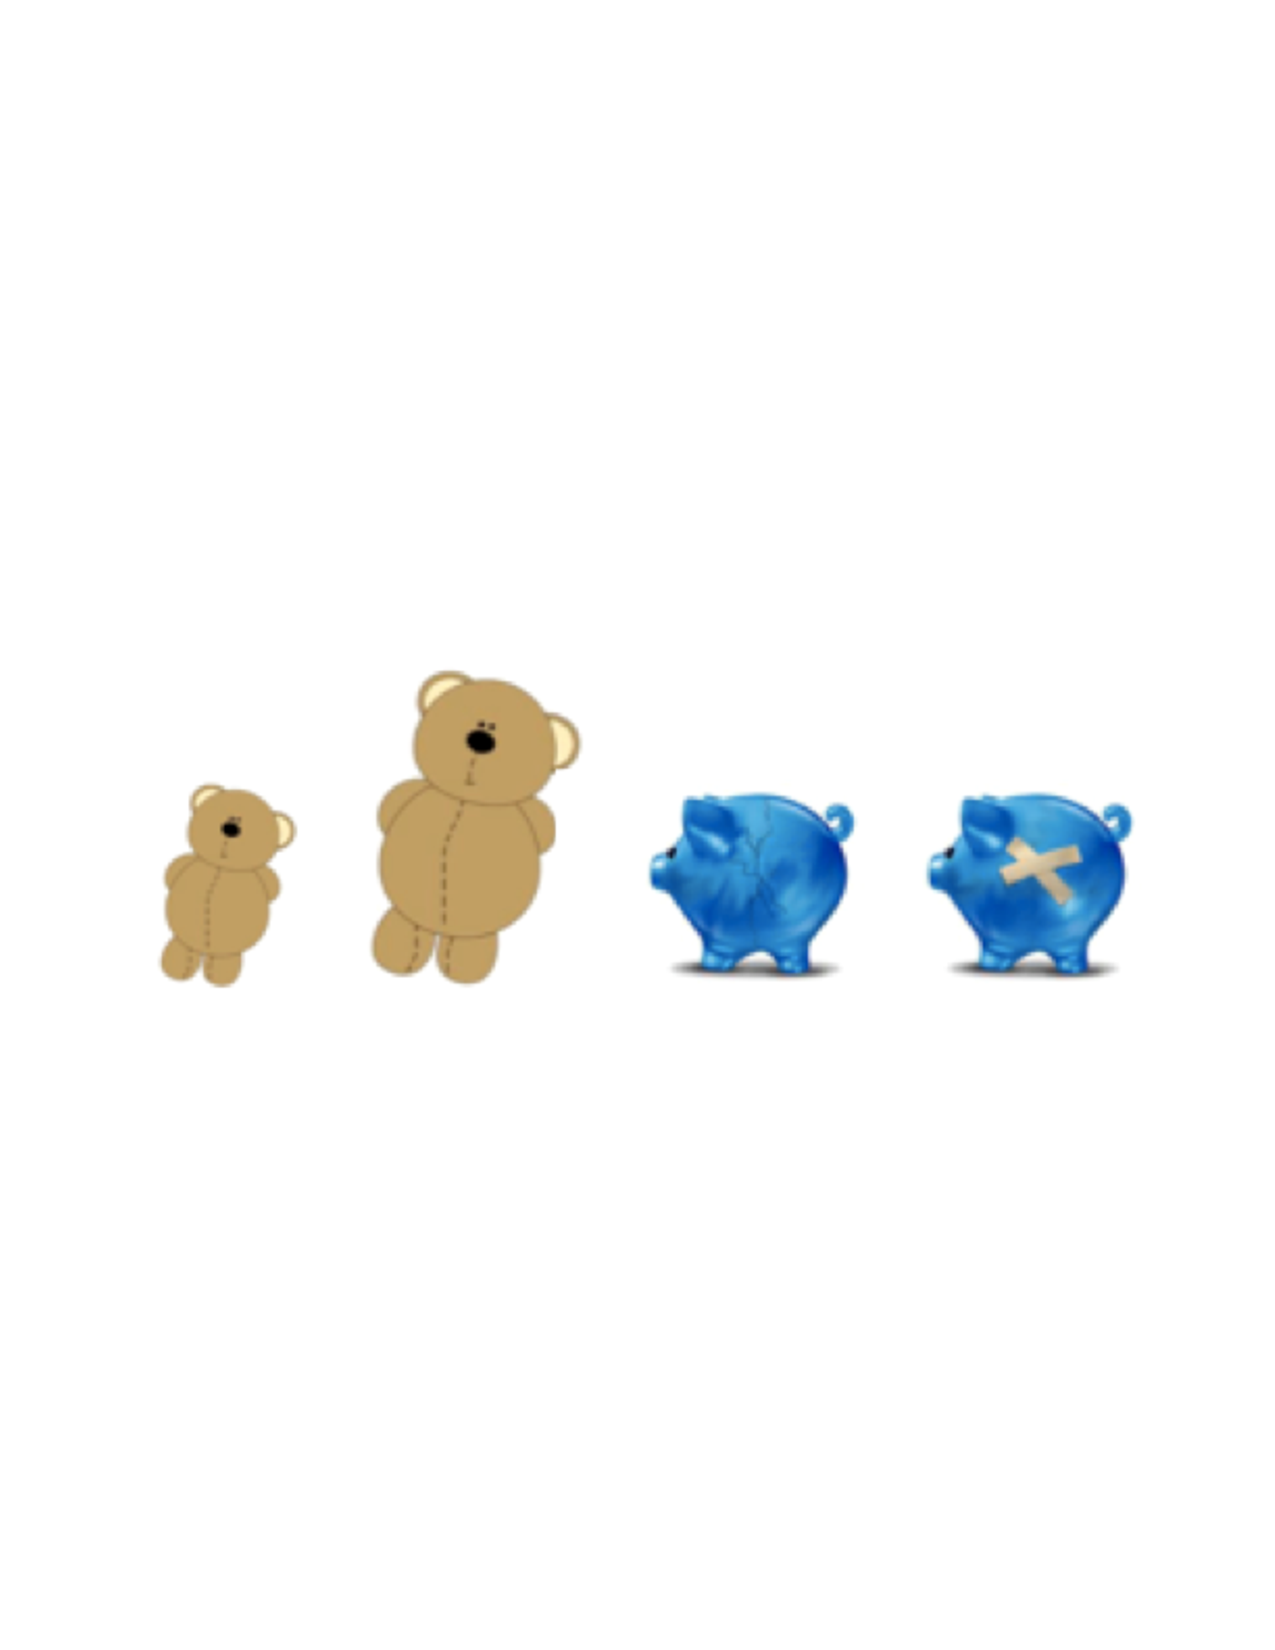
\includegraphics[width=3.5in]{figures/training_demo.pdf} 
    % \vspace{-2in}
    \caption{\label{fig:training_demo} Examples of training pairs used in Experiment 3.  The teddybears depict a size contrast (small -- big) and the piggybanks depict a feature contrast (broken -- fixed).}
  \end{center} 
   \vspace{-3.0ex} 
\end{figure}









\bibliographystyle{apacite2}
\bibliography{ADJ}

\end{document}
